\documentclass{beamer}

\def\Tiny{\fontsize{6pt}{6pt}\selectfont}
\def\supertiny{\fontsize{4pt}{4pt}\selectfont}

\mode<presentation>
{
  \usetheme{Warsaw}
  % \setbeamercovered{transparent}
  \usecolortheme{crane}
}


\usepackage{graphicx, ifthen, listings}

\usepackage[czech]{babel}
% \usefonttheme{professionalfonts}
\usepackage{times}
\usepackage{amsmath}
\usepackage[utf8]{inputenc}
\usepackage{wrapfig}

\usepackage[T1]{fontenc}

\lstset{ basicstyle=\tiny, stringstyle=\ttfamily, showstringspaces=false }

\everymath{\displaystyle}

\setbeamerfont{frametitle}{size=\large}
\setbeamerfont{subsection in toc}{size=\scriptsize}

\makeatletter\newenvironment{blackbox}{%
   \begin{lrbox}{\@tempboxa}\begin{minipage}{0.95\columnwidth}}{\end{minipage}\end{lrbox}%
   \colorbox{black}{\usebox{\@tempboxa}}
}\makeatother

\title[IMF (4)]{Informatika pro moderní fyziky (4)\\vstupní a výstupní soubory pro výpočetní programy}

\author[Franti\v{s}ek HAVL\r{U}J, ORF ÚJV Řež]{Franti\v{s}ek HAVL\r{U}J\\{\scriptsize \emph{e-mail: haf@ujv.cz}}}

\date{akademický rok 2016/2017\\26. října 2016}

\institute[ORF ÚJV Řež]
{ÚJV Řež\\oddělení Reaktorové fyziky a podpory palivového cyklu}

\AtBeginSection[]
{
\begin{frame}<beamer>
\frametitle{Obsah}
\tableofcontents[currentsection,hideothersubsections]
\end{frame}
}

\begin{document}

\begin{frame}
  \titlepage
\end{frame}

\begin{frame}
  \tableofcontents
\end{frame}

\section{Dodělávka z (před)minula: jehla v kupce sena}

\begin{frame}{Zadání}
  \begin{block}{\# 1}
    Adresář plný CSV souborů (stovky souborů) obsahuje data, která jsou záznamy signálů s lineární závislostí.

    V pěti z nich jsou ale poruchy - data ležící zcela mimo přímku.

    Kde?
  \end{block}
\end{frame}

\begin{frame}{Příklad - dobrý signál}
  \begin{center}
      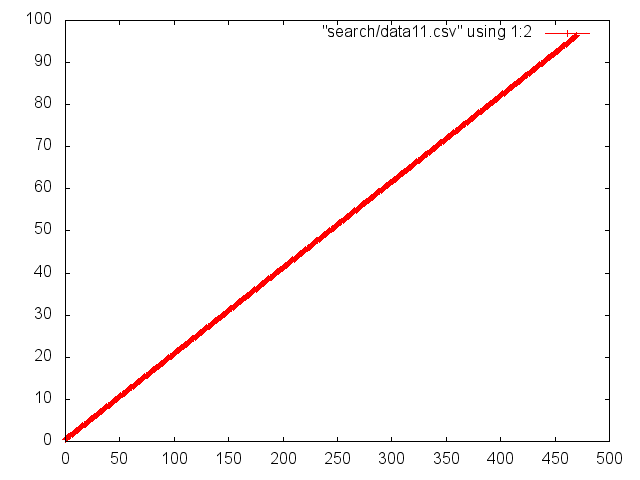
\includegraphics[width=0.6\columnwidth]{search_good}
      \end{center}
\end{frame}
\begin{frame}{Příklad - špatný signál}
  \begin{center}
      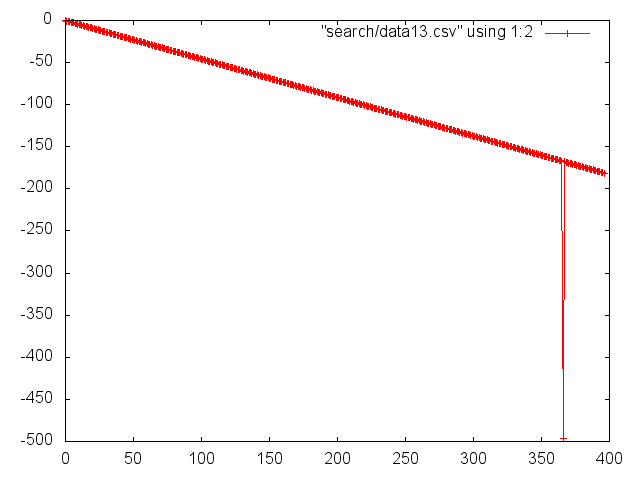
\includegraphics[width=0.6\columnwidth]{search_bad}
      \end{center}
\end{frame}

\begin{frame}{Řešení plně automatické}
  \begin{itemize}
    \item trocha matematiky po inženýrsku
    \item odečtu vhodnou lineární funkci
    \item podívám se na rozdíl mezi minimem a maximem
  \end{itemize}
  nebo
  \begin{itemize}
    \item sleduju rozdíl dvou po sobě jdoucích hodnot
    \item pokud se mi sgn(dx) změní, tak je jasno
  \end{itemize}
\end{frame}

\section{Hrabání listí dělá pořádek (Rake)}

\begin{frame}{Spousta skriptů, spousta zmatku}
  \begin{itemize}
    \item mám jeden projekt/práci a potřebuju udělat víc věcí
    \item zatím jsme měli jeden skript na jednu věc
    \item což skončí hromadou .rb souborů, kde nebudu vědět co dělá který a budu v tom mít trochu zmatek
    \item nehledě na to, že bych mohl chtít sdílet nějakou konfiguraci (jména souborů atd.)
  \end{itemize}
\end{frame}

\begin{frame}{Nástroj Rake}
  \begin{itemize}
    \item alternativa k unixovému MAKE, ale v Ruby (Ruby MAKE = Rake)
    \item nejjednodušší -- nastrkám si do jednoho Rakefile víc úloh (\texttt{task}) a ty pak snadno spustím
    \item složitější -- můžu specifikovat závislosti
  \end{itemize}
\end{frame}

\begin{frame}[fragile]{Rakefile - příklad}
  \begin{block}{obsah Rakefile}
        \scriptsize
    \begin{verbatim}
    desc "rearrange keff into a nice table"
    task :rearrange do
    ...
    end

    desc "find something somewhere"
    task :find do
    ...
    end
    \end{verbatim}
  \end{block}
  \begin{block}{spuštění}
        \scriptsize
    \begin{verbatim}
rake find
rake -T
    \end{verbatim}
  \end{block}
\end{frame}

\begin{frame}[fragile]{Spouštění programů z Ruby}
  Je otrava psát pořád cestu ke gnuplotu a vůbec, takže lze samozřejmě vyrobit rake task:
    \scriptsize
\begin{verbatim}
task :plot do
  system("\"C:/Program Files/gnuplot/bin/gnuplot.exe\" plot1.gp")
end
\end{verbatim}
\end{frame}

\section{Zpracování textu}

\subsection{Obecný rozbor}

\begin{frame}{Problém č. 3: mnoho výpočtů, inženýrova smrt}
  \begin{block}{Zadání}
    Při přípravě základního kritického experimentu je pomocí MCNP potřeba najít kritickou polohu regulační tyče R2.

    Jak se tato poloha změní při změně polohy tyče R1?
  \end{block}
\end{frame}

\begin{frame}{Co máme k~dispozici?}
  \begin{block}{MCNP}
    Pokud připravíme vstupní soubor (v~netriviální formě obsahující polohy regulačních tyčí R1 a R2), spočítá nám keff.
  \end{block}
  Potřebovali bychom ale něco na:
  \begin{enumerate}
    \item vytvoření velkého množství vstupních souborů
    \item extrakci keff z~výstupních souborů
    \item popřípadě na vyhodnocení získaných poloh tyčí a keff
  \end{enumerate}
\end{frame}

\begin{frame}{Pracovní postup}
  \begin{enumerate}
    \item načíst keff z~výstupního souboru MCNP
    \pause
    \item vygenerovat potřebné vstupní soubory
    \pause
    \item vyrobit BAT soubor na spuštění výpočtů
    \pause
    \item načíst výsledky ze všech výstupních souborů do jedné tabulky
    \pause
    \item buď zpracovat ručně (Excel), nebo být Myšpulín a vyrobit skript (úkol s~hvězdičkou)
  \end{enumerate}
\end{frame}

\subsection{Načítání výstupního souboru}

\begin{frame}[fragile]{}
  Nejprve najdeme, kde je ve výstupu z~MCNP žádané keff:
  {\tiny
  \begin{verbatim}
.....
         the k(trk length) cycle values appear normally distributed at the 95 percent confidence level

-----------------------------------------------------------------------------------------------------------------------------------
|                                                                                                                                 |
| the final estimated combined collision/absorption/track-length keff = 1.00353 with an estimated standard deviation of 0.00024   |
|                                                                                                                                 |
| the estimated 68, 95, & 99 percent keff confidence intervals are 1.00329 to 1.00377, 1.00305 to 1.00400, and 1.00289 to 1.00416 |
|                                                                                                                                 |
| the final combined (col/abs/tl) prompt removal lifetime = 1.0017E-04 seconds with an estimated standard deviation of 2.7364E-08 |
.....
  \end{verbatim}
  }
\end{frame}

\begin{frame}{Algoritmus}
  \begin{enumerate}
    \item najít řádek s~keff
    \pause
    \item vytáhnout z~něj keff, takže například:
    \pause
    \item rozdělit podle rovnítka
    \pause
    \item druhou část rozdělit podle mezer
    \pause
    \item vzít první prvek
  \end{enumerate}
\end{frame}


\begin{frame}[fragile]{Realizace (1/5)}
  \scriptsize
  \begin{verbatim}
    keff = nil

    File.foreach("c1_1o") do |line|

    end

    puts keff
  \end{verbatim}
\end{frame}

\begin{frame}[fragile]{Realizace (2/5)}
  \scriptsize
  \begin{verbatim}
    keff = nil

    File.foreach("c1_1o") do |line|
      if line.include?("final estimated combined")

      end
    end

    puts keff
  \end{verbatim}
\end{frame}

\begin{frame}[fragile]{Realizace (3/5)}
  \scriptsize
  \begin{verbatim}
    keff = nil

    File.foreach("c1_1o") do |line|
      if line.include?("final estimated combined")
        a = line.split("=")

      end
    end

    puts keff
  \end{verbatim}
\end{frame}

\begin{frame}[fragile]{Realizace (4/5)}
  \scriptsize
  \begin{verbatim}
    keff = nil

    File.foreach("c1_1o") do |line|
      if line.include?("final estimated combined")
        a = line.split("=")
        b = a[1].split

      end
    end

    puts keff
  \end{verbatim}
\end{frame}

\begin{frame}[fragile]{Realizace (5/5)}
  \scriptsize
  \begin{verbatim}
    keff = nil

    File.foreach("c1_1o") do |line|
      if line.include?("final estimated combined")
        a = line.split("=")
        b = a[1].split
        keff = b[0]
      end
    end

    puts keff
  \end{verbatim}
\end{frame}


\section{Automatizace tvorby vstupů}

\begin{frame}[fragile]{Určení poloh tyčí}
  Ve vstupním souboru si najdeme relevantní část:
  \scriptsize
  \begin{verbatim}
    c ---------------------------------
    c polohy tyci (z-plochy)
    c ---------------------------------
    c
    67 pz 47.6000    $ dolni hranice absoberu r1
    68 pz 40.4980    $ dolni hranice hlavice r1
    69 pz 44.8000    $ dolni hranice absoberu r2
    70 pz 37.6980    $ dolni hranice hlavice r2
  \end{verbatim}
\end{frame}

\begin{frame}[fragile]{Výroba šablon}
  Jak dostat polohy tyčí do vstupního souboru? Vyrobíme šablonu, tzn nahradíme
  \begin{verbatim}
    67 pz 47.6000    $ dolni hranice absoberu r1
  \end{verbatim}
  \pause
  nějakou značkou (\emph{placeholder}):
  \begin{verbatim}
    67 pz %r1%    $ dolni hranice absoberu r1
  \end{verbatim}
\end{frame}

\begin{frame}{Chytáky a zádrhele}
  \begin{itemize}
    \item kromě samotné plochy konce absorbéru je nutno správně umístit i z-plochu konce hlavice o 7,102 cm níže
    \item obecně je na místě ohlídat si, že placeholder nebude kolidovat s ničím jiným
  \end{itemize}
  Doporučené nástroje jsou:
  \begin{itemize}
    \item již známá funkce \texttt{sub} pro nahrazení jednoho řetězce jiným
    \item pro pragmatické lenochy funkce \texttt{File.read} načítající celý soubor do řetězce (na což nelze v Pascalu ani pomyslet)
    \item možno ovšem použít i \texttt{File.readlines} (v čem je to lepší?)
  \end{itemize}
\end{frame}

\begin{frame}[fragile]{Realizace}
  \scriptsize
  \begin{verbatim}
    DELTA = 44.8000 - 37.6980

    template = File.read("template")
    (0..10).each do |i1|
      (0..10).each do |i2|
        r1 = i1 * 50
        r2 = i2 * 50
        File.open("inputs/c_#{i1}_#{i2}", "w") do |f|
          s = template.sub("%r1%", r1.to_s)
          s = s.sub("%r1_%", (r1 - DELTA).to_s)
          s = s.sub("%r2%", r2.to_s)
          s = s.sub("%r2_%", (r2 - DELTA).to_s)
          f.puts template
        end
      end
    end
  \end{verbatim}
\end{frame}

\subsection{Zápis všech výsledků do tabulky}

\begin{frame}{Jak na to}
  Máme všechno, co potřebujeme:
  \begin{itemize}
    \item načtení keff z~jednoho výstupního souboru (\texttt{File.foreach}, \texttt{include} a \texttt{split})
    \item procházení adresáře (\texttt{Dir.each})
    \item zápis do souboru (\texttt{File.open} s~parametrem \texttt{w})
  \end{itemize}
  Takže už to stačí jen vhodným způsobem spojit dohromady!
\end{frame}

\begin{frame}[fragile]{Realizace}
  \scriptsize
  \begin{verbatim}
    Dir["*o"].each do |filename|
      keff = nil

      File.foreach(filename) do |line|
        if line.include?("final estimated combined")
          a = line.split("=")
          b = a[1].split
          keff = b[0]
        end
      end

      puts "#{filename} #{keff}"
    end
  \end{verbatim}
\end{frame}

\begin{frame}[fragile]{Výstup}
  Výsledkem je perfektní tabulka:
  {\scriptsize
  \begin{verbatim}
    outputs/c_0_0o 0.94800
    outputs/c_0_10o 0.99800
    outputs/c_0_1o 0.94850
    outputs/c_0_2o 0.95000
    outputs/c_0_3o 0.95250
    outputs/c_0_4o 0.95600
    ...
  \end{verbatim}}
  Hloupé je, že nikde nemáme tu polohu tyčí.
\end{frame}


\begin{frame}[fragile]{Chytrá horákyně}
  ... by jistě vyrobila toto:
  {\scriptsize
  \begin{verbatim}
    0 0 0.94800
    0 10 0.99800
    0 1 0.94850
    0 2 0.95000
    0 3 0.95250
    0 4 0.95600
    ...
  \end{verbatim}
  }
  Nápovědou je funkce \texttt{split} (podle podtržítka) a funkce \texttt{to\_i} (co asi dělá?)
\end{frame}

\begin{frame}[fragile]{Realizace chytré horákyně}
  \scriptsize
  \begin{verbatim}
    Dir["outputs/*o"].each do |filename|
      keff = nil

      File.foreach(filename) do |line|
        if line.include?("final estimated combined")
          a = line.split("=")
          b = a[1].split
          keff = b[0]
        end
      end

      s = filename.split("_")
      puts "#{s[1].to_i} #{s[2].to_i} #{keff}"
    end
  \end{verbatim}
\end{frame}

\subsection{Co dál?}

\begin{frame}{Navážeme na úspěchy z minulých týdnů}
  \begin{itemize}
    \item vykreslit graf! pro každou z 11 poloh R1 jedna čára (závislost keff na R2)
    \item (= csv soubor, gnuplot, znáte to)
    \item najít automaticky kritickou polohu R2 pro každou z 11 poloh R1
    \item a zase graf... (kritická poloha R2 v závislosti na R1)
  \end{itemize}
\end{frame}

\begin{frame}{A to je vše, přátelé!}
  \begin{center}
    
\includegraphics[width=0.8\textwidth]{looney_tunes}
  \end{center}
\end{frame}

\end{document}
